\documentclass[tikz]{standalone}
\usepackage{bm}
\begin{document}
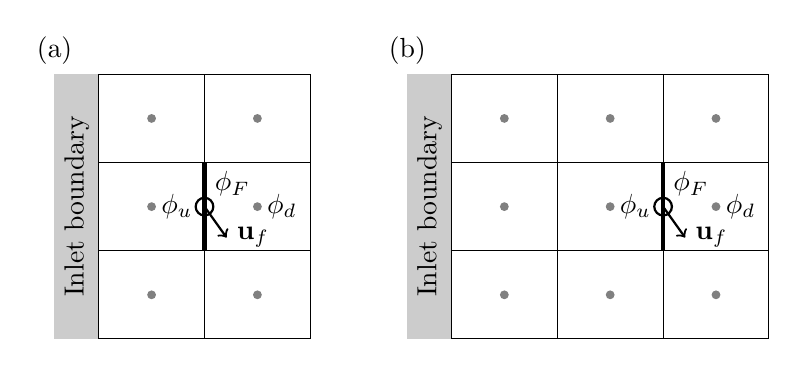
\begin{tikzpicture}[
  scale=0.56,
  cpnt/.style={fill=gray},
]

\node [above] at (-1,6) {(a)};
\draw (-1,0) [fill=black!20,black!20] rectangle (0,6) node [midway,black] {\rotatebox{90}{Inlet boundary}};
\draw (0,0) rectangle (4.8,6);
\draw (0,2) -- (4.8,2);
\draw (0,4) -- (4.8,4);
\draw (0,0) -- (0,6);
\draw (2.4,0) -- (2.4,6);

\draw [ultra thick] (2.4,2) -- (2.4,4);
\draw [thick] (2.4,3) circle [radius=0.2] node [anchor=south west] {$\phi_F$};
\draw [thick, ->] (2.4,3) -- (2.9,2.3) node [anchor=west] {$\mathbf{u}_f$};

\path [cpnt] (1.2,1) circle [radius=0.1];
\path [cpnt] (1.2,3) circle [radius=0.1] node [right] {$\phi_u$};
\path [cpnt] (1.2,5) circle [radius=0.1];

\path [cpnt] (3.6,1) circle [radius=0.1];
\path [cpnt] (3.6,3) circle [radius=0.1] node [right] {$\phi_d$};
\path [cpnt] (3.6,5) circle [radius=0.1];

\begin{scope}[shift={(8,0)}]
\draw (-1,0) [fill=black!20,black!20] rectangle (0,6) node [midway,black] {\rotatebox{90}{Inlet boundary}};
\node [above] at (-1,6) {(b)};

\draw (0,0) rectangle (7.2,6);
\draw (0,2) -- (7.2,2);
\draw (0,4) -- (7.2,4);
\draw (0,0) -- (0,6);
\draw (2.4,0) -- (2.4,6);
\draw (4.8,0) -- (4.8,6);

\draw [ultra thick] (4.8,2) -- (4.8,4);
\draw [thick] (4.8,3) circle [radius=0.2] node [anchor=south west] {$\phi_F$};
\draw [thick, ->] (4.8,3) -- (5.3,2.3) node [anchor=west] {$\mathbf{u}_f$};

\path [cpnt] (1.2,1) circle [radius=0.1];
\path [cpnt] (1.2,3) circle [radius=0.1];
\path [cpnt] (1.2,5) circle [radius=0.1];

\path [cpnt] (3.6,1) circle [radius=0.1];
\path [cpnt] (3.6,3) circle [radius=0.1] node [right] {$\phi_u$};
\path [cpnt] (3.6,5) circle [radius=0.1];

\path [cpnt] (6.0,1) circle [radius=0.1];
\path [cpnt] (6.0,3) circle [radius=0.1] node [right] {$\phi_d$};
\path [cpnt] (6.0,5) circle [radius=0.1];
\end{scope}

\end{tikzpicture}
\end{document}
